\PassOptionsToPackage{table}{xcolor}

\documentclass[journal = enfuem, manuscript =  article]{achemso}
\usepackage[utf8]{inputenc}
\usepackage{natbib} \renewcommand{\bibname}{References}
\bibliographystyle{agsm}
\setcounter{tocdepth}{4}
\setcounter{secnumdepth}{4}
%% use bib entries
\usepackage{usebib}
\newbibfield{institution}
\bibinput{ref}
%% Nomenclature
\usepackage{nomencl}
\makenomenclature
\setlength{\nomlabelwidth}{.2\textwidth}
% NOMENCLATURE groups
% -----------------------------------------
\usepackage{etoolbox}
\renewcommand\nomgroup[1]{%
  \item[\bfseries
  \ifstrequal{#1}{A}{Abbreviations}{%
  \ifstrequal{#1}{S}{Symbols}{%
  \ifstrequal{#1}{O}{Other Symbols}{}}}%
]}
% -----------------------------------------
\usepackage[section]{placeins} % gives you \FloatBarrier so all floats are printed by then
% \usepackage{fourier} 
% \usepackage{array}
\usepackage{makecell} % gives you \thead and \makecell in which you can use line breaks \\
\renewcommand\theadalign{bc}
\renewcommand\theadfont{\bfseries}
\renewcommand\theadgape{\Gape[4pt]}
\renewcommand\cellgape{\Gape[4pt]}
\usepackage{xcolor}
% \PassOptionsToPackage{table}{xcolor}
%% Make index
\usepackage{makeidx}
\makeindex
%% color boxes around text
\usepackage{tcolorbox}
%% images and graphics
\usepackage{subcaption}
\usepackage{graphicx}
\usepackage{adjustbox}

% \graphicspath{ {./img/} }
% %% TABLES AND TABLE COLORS
% \usepackage{tabu}
% \usepackage{longtable}
%% American Mathematical Society packages
\usepackage{amsmath}
\usepackage{amsfonts}
\usepackage{amssymb}
\usepackage{amsthm}
%% Print program code
\usepackage{listings}
%% Better looking tables
\usepackage{booktabs} % provides \cmidrule[2pt](lr){1-2}
\usepackage{multirow}
\newcommand{\tabitem}{\quad\llap{\textbullet}~~}
%% Handle formatting of numbers and units
\usepackage{sistyle}
%% hyperlinks throughout the doc
\usepackage{hyperref}
\hypersetup{
    colorlinks=true,
    citecolor={blue},
    linkcolor={blue}
}
%% Add quotes at the beginning of a chapter
\usepackage{epigraph}
\setlength{\epigraphwidth}{.5\textwidth}
%% Allows to write Unicode e.g., Blåbær syltetøy
% \usepackage{ucs}
%% correctly typeset chemical compounds e.g., \ce{H3PO4}
\usepackage[version=4]{mhchem}
%%%%%%%%%%%%%%%% OTHER PACKAGES
\usepackage{ textcomp, gensymb } % °C
% -----------------------------------------
%% Paper info %%
% -----------------------------------------
\title[Hybrid Green Gels]
{HyGreGel (Hybrid Green Gels), a New Class of Polymer Gels Made of Functionalized Silica Nanoparticles for Conformance Control}
% ===
\author{Bahador Najafiazar}
\email{bahador.najafiazar@ntnu.no}
\affiliation{Dept. of Geoscience and Petroleum, Norwegian University of Science and Technology}
% ===
\author{Dag Wessel-Berg}
\email{dag.wessel-berg@ntnu.no}
\affiliation[]{Dept. of Mathematical Sciences, Norwegian University of Science and Technology}
\alsoaffiliation{SINTEF Industry,  Norway}
% ===
\author{Per Eirik Bergmo}
\email{per.bergmo@sintef.no}
\affiliation{SINTEF Industry,  Norway}
% ===
\author{Christian Rone Simon}
\email{christian.r.simon@sintef.no}
\affiliation{SINTEF Industry,  Norway}
% ===
\author{Juan Yang}
\email{juan.yang@sintef.no}
\affiliation{SINTEF Industry,  Norway}
% ===
\author{Ole Torsæter}
\email{ole.torsater@ntnu.no}
\affiliation{Dept. of Geoscience and Petroleum, Norwegian University of Science and Technology}
% ===
\author{Torleif Holt}
\email{torleif.holt@sintef.no}
\affiliation{SINTEF Industry,  Norway}




\begin{document}
\begin{abstract}
High water production is typically a major problem late in the life cycle of a water flooded hydrocarbon reservoir. Reservoir heterogeneity plays a significant role in creating this problem. An example is highly permeable zones and streaks in the reservoir, the so-called ``thief zones". These zones attract the injected water and result in early water breakthrough, hence high water cuts in production wells. 

One solution to this problem is blocking the thief zones. As a result, the injected water will be diverted from channels with high water flow into other (potentially oil-bearing) areas of the reservoir. The prospective end result is reduced water production and increased oil production.  This may be achieved by deep placement of polymer gels in the reservoir. 

Deep placement of gels is challenging. This is owing to the fact that fully formed gels cannot be transported through porous media deep into the formation. A workaround is to transport gel constituents, \textit{i.e.}, polymer and a cross-linking agent, to the proper area in the reservoir before gelling begins. This requires a delay in gelling time at elevated temperatures of the reservoir. Moreover, the gel constituents must be environmentally sound.

This work is part of the HyGreGel (Hybrid Green nano-Gels) project. As a result of this project gel systems with delayed gelation times were developed and tested. The objective was to enable the chemicals to reach the desired position in the reservoir before gelation would prohibit further transport. Furthermore, mechanisms for transport and reaction of the gel constituents were described and modelled. 

\end{abstract}

\section{Introduction}
It is becoming more and more challenging to meet the ever-increasing demand for petroleum. Most of the existing major oilfields are already at a mature stage and the number of new significant discoveries per year is decreasing. Therefore, at this point in time, it is crucial to focus on methods of improving petroleum production from existing reservoirs. A big subset of such methods fall under the category of Enhanced Oil Recovery (EOR).

Challenges and technology gaps within EOR, which need to be addressed in the coming research programs, have been identified in the OG21 strategy document on ``Exploration and Increased Recovery" \citep{OG21}: In particular, there is a need for more cost-efficient EOR chemicals, and to assure environmentally acceptable methods to avoid unwanted discharge to sea. Improved petroleum resource exploitation by EOR has also been given special attention in a report on increased recovery in the Norwegian Continental Shelf by the Norwegian Department of Oil and Energy \citep{Am2010}. There is therefore a clear need for increased competence in new technologies in the field of EOR. 

There has recently been an increasing interest in applying nanotechnology to EOR but still many topics are uncovered. Nanotechnology, which has mainly been developed in mechanical engineering, medicine and biological sciences, is expected to have a large potential for EOR applications. This technology has a wide range of applications relevant to EOR, from employing general concepts and principles of nanotechnology, to advanced reservoir monitoring using nano-sensors and nano-analysis, to more specific technologies which make up for the shortcomings in traditional EOR methods \citep{Fletcher2010, Ayatollahi2012, Cocuzza2011}. The latter includes tailoring chemical molecules for more efficient EOR, as well as smart and more effective delivery of EOR agents. Such technologies as efficient drug delivery in the human body may be applied to improve efficiency in chemical flooding.

This work is part of the HyGreGel (Hybrid Green nano-Gels) project carried out at SINTEF Industry and Norwegian University of Science and Technology. It addresses the need for more efficient water diversion techniques by improved in-depth placement of gelling chemicals to increase waterflood recovery and reduce unwanted water circulation in heterogeneous reservoirs. The project recognizes the environmental challenges using chemicals and emphasizes the development of green chemical systems for such applications.

Incremental recovery from water diversion is generally expected to be merely 2\% above standard water flooding \citep{OG21}. The main objective of this work is thus to improve incremental recovery from water diversion by developing and testing innovative hybrid (polymer + nanoparticle) gels.

\subsection{Hybrid Materials for Delayed Gellation}
Hybrid materials based on FunzioNano\texttrademark (FN) nanoparticles were used in this work. FN partciles, which are developed at  the  Department  of  Materials  and  Nanotechnology at  SINTEF  Industry (DMN), are nanoparticles with functional groups having the ability to react with polymers causing cross-binding and gelling. 

FunzioNano cross-linker and polymer are injected as a formulation at the same time. Hydrolysis within the requested time window leads to de-blocking of the functional groups and thereafter fast and efficient gelation by cross-linking of FunzioNano and polymer, e.g. through ionic bond formation between amine functionalities on FunzioNano and carboxylic functionalities on cellulose.

The time window for de-blocking FunzioNano can be adjusted by the type and the amount of hydrolysis catalyst. As an additional benefit cross-linked FunzioNano and polymer can provide a more hydrophobic gel than the components themselves. Motion of water could therefore be more efficiently hindered than motion of produced oil which would be suitable for partially blocking gels that can transport the remaining oil. FunzioNano can to a significant extent be manufactured from renewable resources. In case of un-desired spill, FunzioNano is degradable after being highly diluted with water. Computer modelling of the degradability of highly diluted FunzioNano was previously performed in collaboration with Université de Savoie, France \citep{Neyertz2012,Neyertz2013}.

The first gelation tests at the Department of Exploration and Reservoir Technology at SINTEF Industry (DER) with active FN particles and polymer revealed that it was difficult to form gels with cellulose based polymer but strong gels were formed with partially hydrolyzed polyacrylamide, HPAM. A low molecular weight HPAM was chosen as the base polymer for the following studies. DER followed two approaches in synthesizing FN-based particles. 
    
    Approach 1 --- The reactive groups of the FN particles were blocked to prevent instant cross binding with the polymer. Then, as a time dependent event, the blocked sites were activated by slow hydrolysis enabling cross-linking, viscosity increase and eventually gel formation.
    
    Approach 2 --- Only parts of the active sites were deactivated. DER found that by partially deactivation of the active sites the formation of gel was controlled to vary from several days to several months.
    
Both types of FN particles synthesized by DER were tested in bulk conditions. Their reactivity was tested by measuring viscosity and gel formation as a function of time at 80~\celsius~ in synthetic sea water at anaerobic conditions. Tested systems were kept in reaction vials and eventually the most promising system  was selected for \emph{in situ} gelling experiments.
    
\subsection{Polyelectrolyte Complexes for Delayed Gellation}
As a second approach for delayed gellation, Polyelectrolyte complexes (PEC) where used. PEC can be made by mixing a polycation with a polyanion. By incorporating a cross-binder into the polyelectrolyte complex a delayed gel formation can be obtained. In the original PEC recipe \ce{Cr^3+} was used as cross-binder. As active FN particles are also polycations, the original polycation was replaced by active FN. Initial tests indicated that this could be a viable approach.

A research group at Texas A\&M\footnote{The research was originally conducted at University of Kansas. However, since Professor Jenn-Tai Liang, one of the contributors to this project and HyGreGel, later moved to Texas A\&M University, we will call it a Texas A\&M recipe here.} has developed a technology to delay gelation of HPAM based on PEC and \ce{Cr^{3+}}. Only a few works have been published on their results \citep{Cordova2008,Johnson2010}. Figure \ref{cht:jennTai} shows an example of a system with delayed gelation based on Texas A\&M technology. As shown in the figure, the viscosity of the solution only increased marginally for the first 50 days after preparation. Then after 50 days, a sudden viscosity increase of several orders of magnitude was observed over a 10 day period.

\begin{figure}
    \centering
    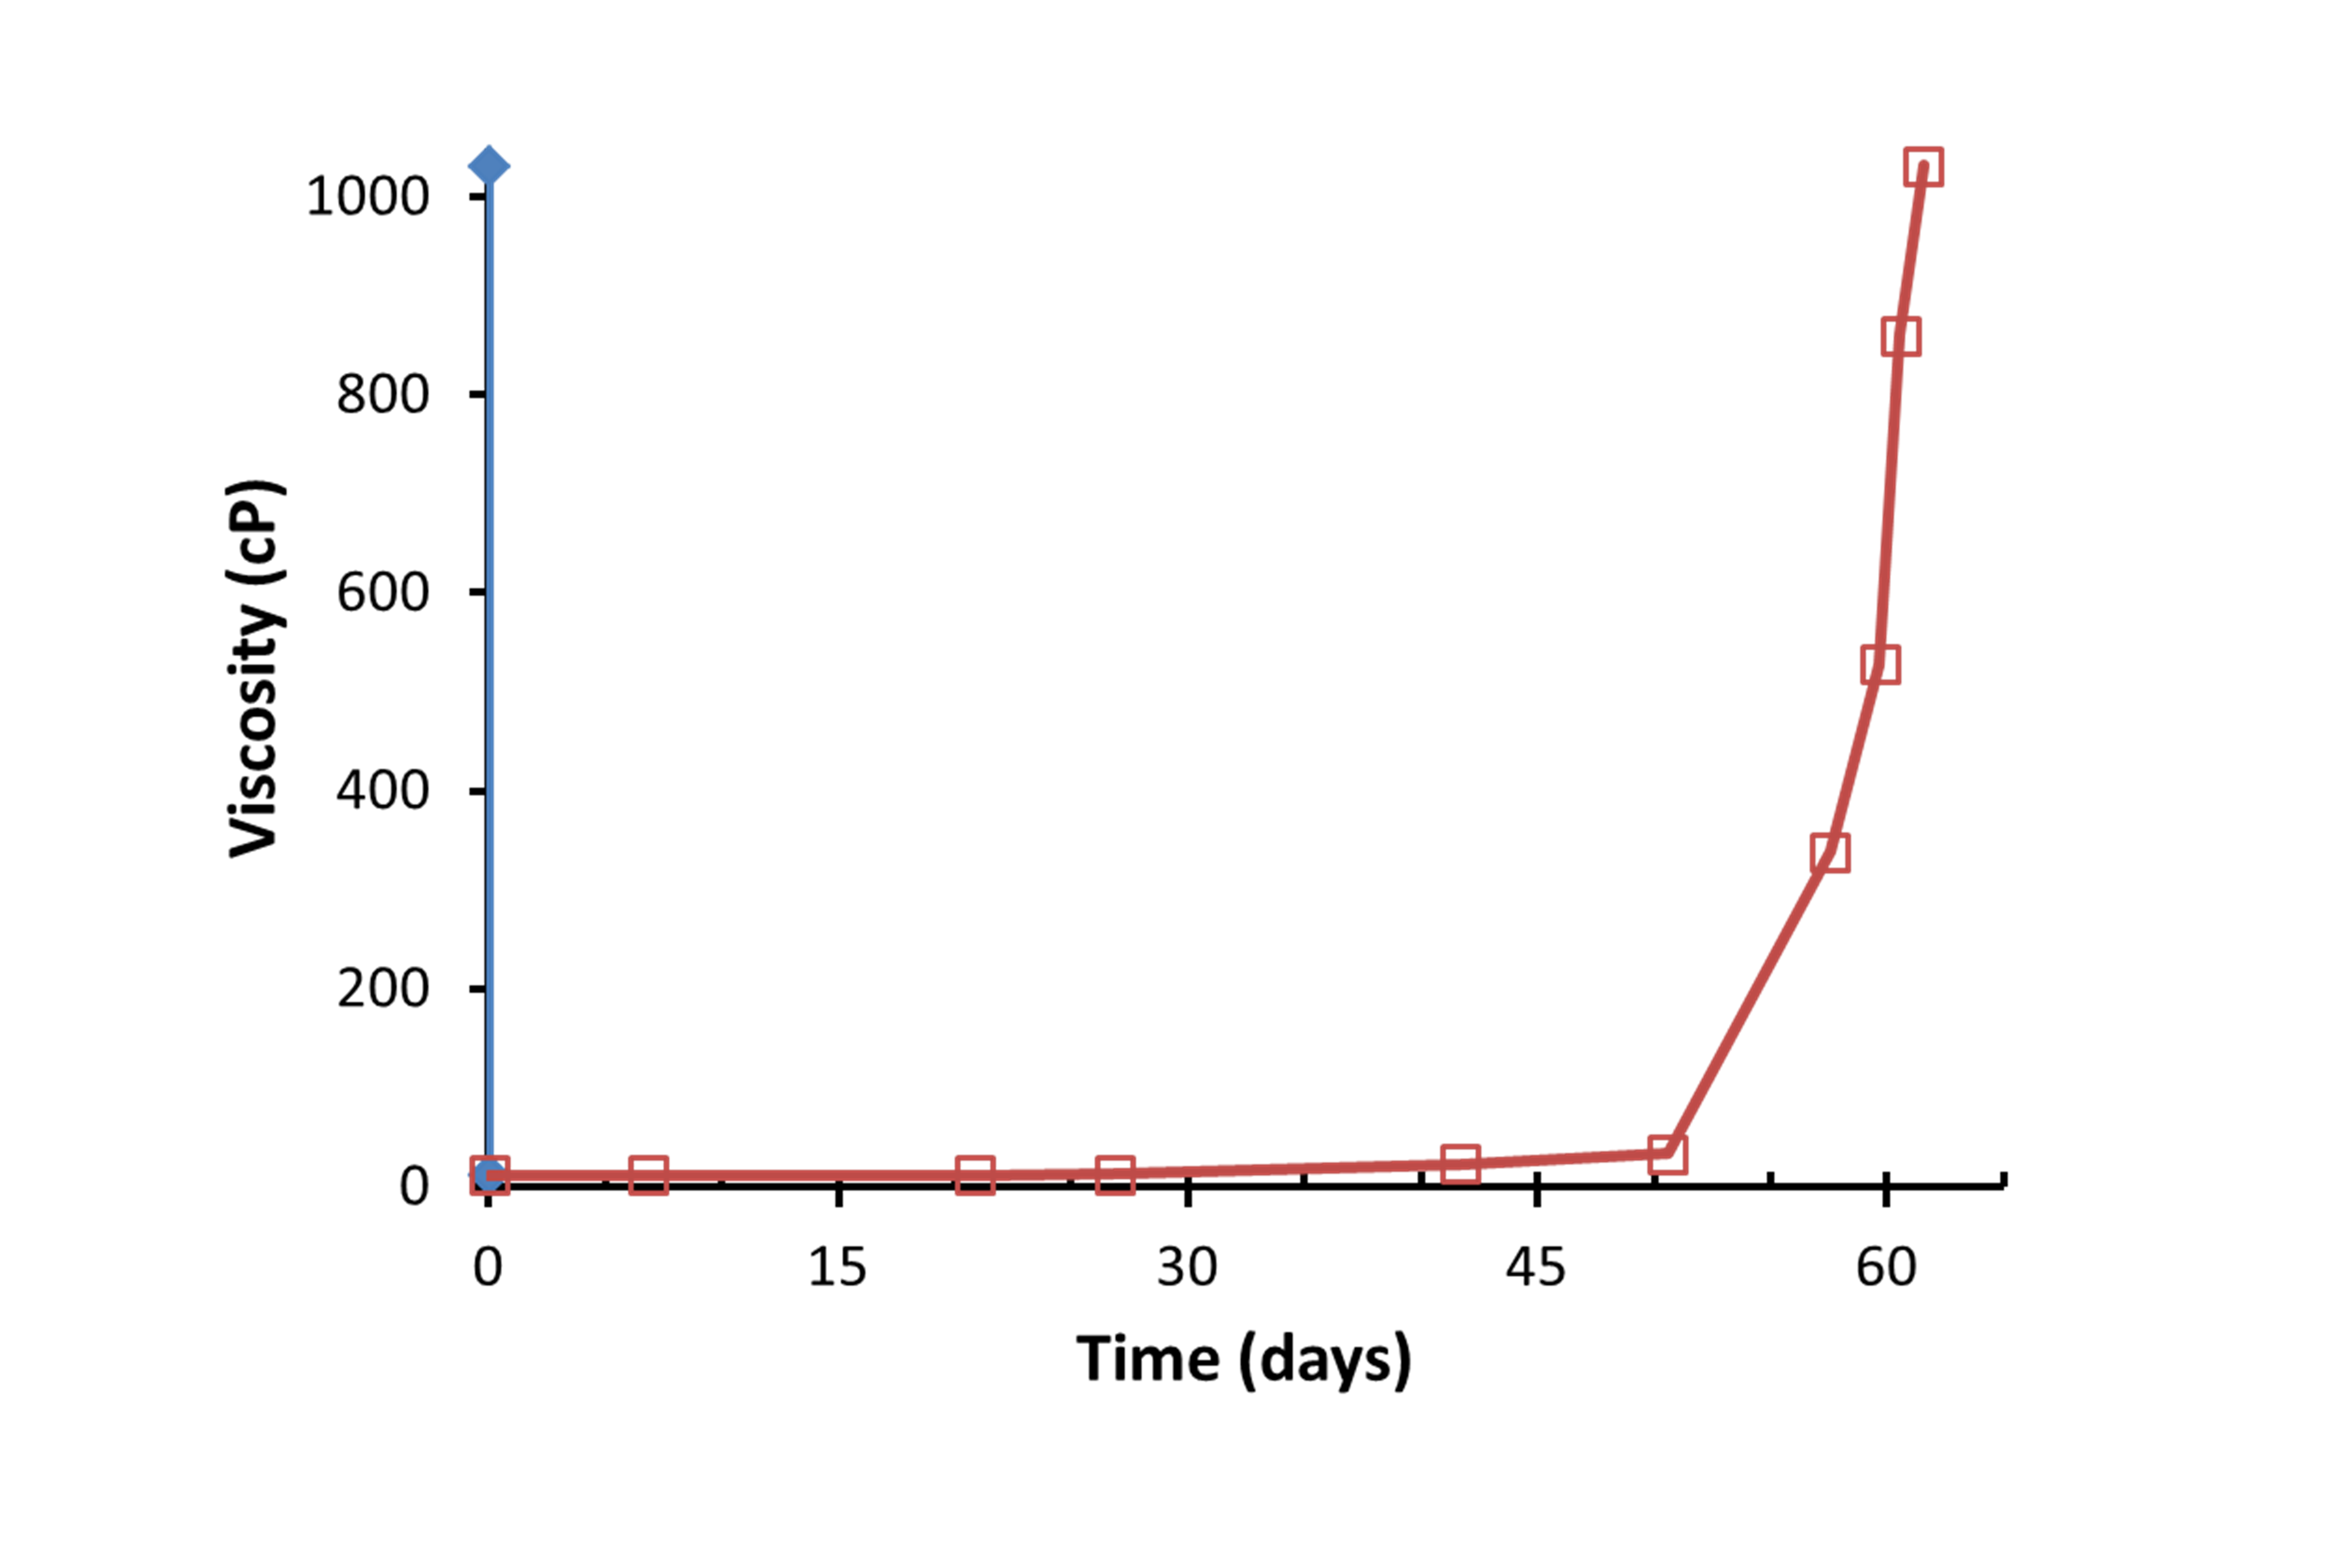
\includegraphics[width=.75\textwidth]{fig/jennTai.png}
    \caption{System with delayed gelation based on Texas A\&M technology \citep{Cordova2008}}
    \label{cht:jennTai}
\end{figure}
    
Samples of different basic systems were prepared for measurement of viscosity development with time. This included systems with only \ce{Cr^3+}-ions as cross-linker, systems based on the original Texas A\&M recipe \citep{Cordova2008} and systems with active FN. Polymers of different molecular weight were used.
    
\subsection{Transport Properties of Nanoparticles and Polymers in Porous Media}
Several core flooding experiments were conducted where deactivated FN particles and polymer were injected both separately and in mixtures into two sets of sandstones, namely Berea and Bentheimer. The results indicate that polymer adsorption\index{adsorption}, polymer retention\index{retention} and inaccessible pore volume \index{inaccessible pore volume} (IPV) were generally reduced by the presence of nanoparticles. Adsorption, total retention and IPV were significantly higher in Berea compared to Bentheimer, for both polymer and nanoparticles. Adsorbed or otherwise retained polymer during injection was not released during following water floods, while the retained nanoparticles were partly released during subsequent water floods. Nanoparticles had negligible effect on rock permeability, while polymer significantly reduced rock permeability.

\subsection{Numerical Model}
A numerical model in was developed and tested with results from the core flooding experiments with deactivated FN particles and polymer. Simulations were also run using a synthetic data set where polymer viscosity depends on polymer concentration and the concentration and age of the injected nanoparticles (the time passed since injection).

% %%%%%%%%%%%%%%%%%%%%%
% EXPERIMENTAL
\section{Experimental}
\subsection{PEC Nanogels}
\textbf{Gels with \ce{Cr^{3+}} as crosslinker.}
Three different polymers (all HPAM) were used in the experiments as summarized in Table \ref{tab:crGels}, where the product names, the producers and the approximate molecular weights are given. The concentrations used are also given. The polymers were always dissolved in synthetic sea water, SSW (cf. Table \ref{tab:sswComp}). The exact molecular weight of Flopaam 5115 VHM is not known but assumed to be in the order of 12 - 15 MDa.

\begin{table} 
\centering
\caption{Basic rock parameters and additives used in the experiments.}
\label{tab:crGels} % table 5.1
\begin{tabular}{c c c c } 
\toprule
\textbf{Name} & \textbf{Producer} & \textbf{MW} & \textbf{Concentration} \\ 
&& [MDa] & [wt\%]   \\
\midrule 
Alcoflood 254 S     & BASF    & 0.5 & 0.5, 1.0 and 2.0\\
Alcomer 24 UK       & BASF    & 6 & 0.25, 0.5, 1.0 and 2.0  \\ 
Flopaam 5115 VHM    & SNF Floerger    & 12+ & 0.5, 1.0 and 2.0  \\ 
\bottomrule
\end{tabular}
\end{table}

\begin{table} 
\centering
\caption{Composition of synthetic seawater (SSW)}
\label{tab:sswComp} 
\begin{tabular}{r c } 
\toprule
\textbf{Salt} & \textbf{Concentration} \\
& [g/l]\\
\midrule 
\ce{NaCl}       & 23.612\\
\ce{CaCl2.2H2O} & 1.911 \\ 
\ce{MgCl2.2H2O} & 9.149 \\ 
\ce{KCl}        & 0.746 \\
\ce{Na2SO4}     & 3.407 \\ 
\bottomrule
\end{tabular}
\end{table}

\textbf{Polyelectrolyte complexes according to the Texas A\&M recipe \citep{Johnson2010}.}
A few tests were conducted with PEC systems made after the recipe by Johnson et el \citep{Johnson2010}, in order to reproduce similar results. In this recipe, in addition to the polymer and cross binder \ce{Cr^3+} the main constituents are dextran sulphate (DS) \index{dextran sulfate} and polyethyleneimine (PEI)\index{polyethyleneimine}. The structure of the two polyelectrolytes are shown in Figure \ref{fig:pei}. Each molecule consists of n repeated units, but n is different for the two components. 1 wt.\% of both components in pure water were prepared for making PEC solutions by adding 15.39 g of DS solution to 34.28 g of PEI solution under vigorous stirring. The DS solution was added quickly as a ``shot" by use of a syringe.

\begin{figure}[h]
    \centering
    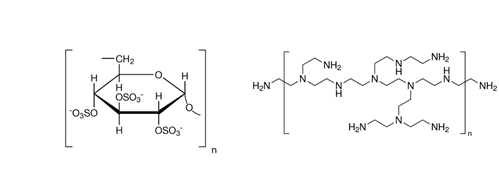
\includegraphics[width=\textwidth]{fig/pei.png}
    \caption{Structures of amine POSS (left) and PVS (right).}
    \label{fig:pei}
\end{figure}    

 
After approximately one minute of stirring, 1.13 g of a 10 wt.\% \ce{CrCl3.6H2O} was added. The final solution was made by first mixing 5.38 g of a 4 wt.\% Alcomer 24 UK solution (in SSW\index{synthetic sea water}) with 25.35 g of SSW. Next, this polymer solution was mixed with 12.32 g of the PEC solution. The concentration of polymer and \ce{Cr^{3+}} in the final solution were 0.499 wt.\% and 129 ppm, respectively. The samples were aged at 50~\celsius. The sample series was named Series 10.

Two more series of polymer/PEC solutions were made using 0.498 wt.\% and 0.490 wt.\% of Alcomer 24 UK (Series 35) and Flopaam 5115 VHM (Series 36), respectively. The composition of the PEC was as described above. The concentrations of \ce{Cr^{3+}} in the two solutions were 119 ppm and 115 ppm. The solutions were aged at 80~\celsius. Yet another two systems were made in an equivalent manner using Alcomer 24 UK, but with reduced concentrations of \ce{Cr^{3+}} (60 ppm in Series 42 and 41 ppm in Series 47).

\textbf{Polyelectrolyte complexes based on amine POSS.}
In PECs based on amine POSS the polycation PEI was replaced by the nanoparticle which also contains amine groups. As suggested by researchers at Texas A\&M the DS was replaced by the polyanion polyvinyl sulfonate (PVS). Series 17 through 20 were made using this method (Table \ref{tab:polyPecComp}). The structure of PVS is also shown in Figure \ref{fig:pvs}.

\begin{figure}[h]
    \centering
    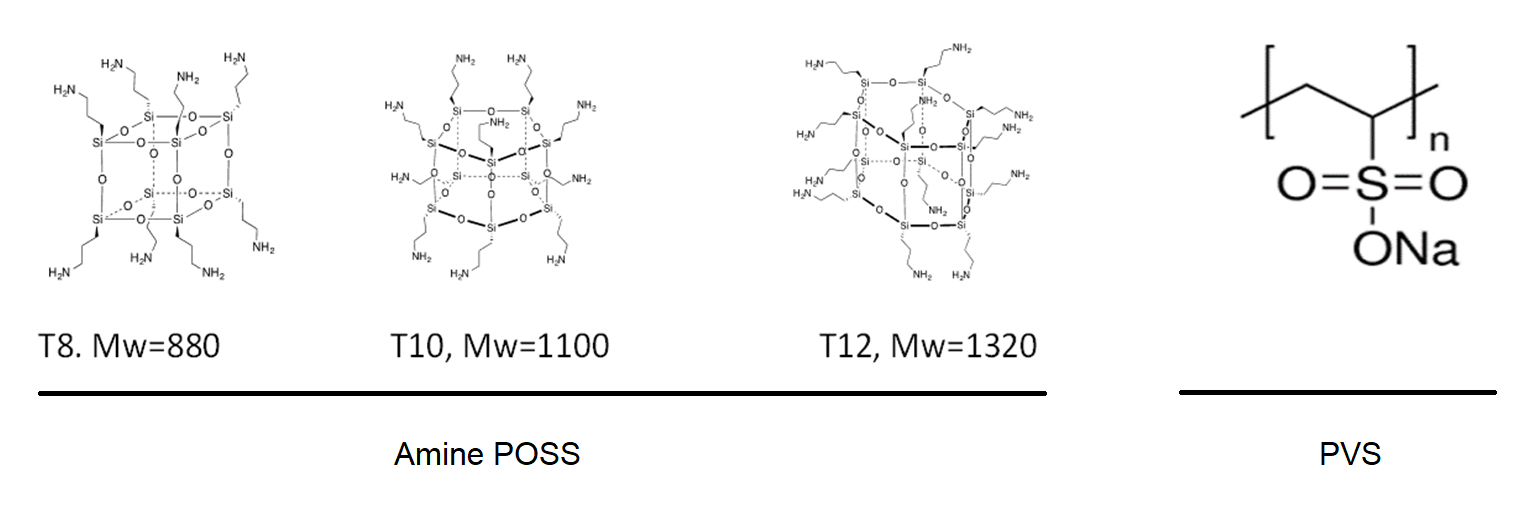
\includegraphics[width=\textwidth]{fig/pvs.png}
    \caption{Structures of amine POSS (left) and PVS (right).}
    \label{fig:pvs}
\end{figure}

The cores of the amine POSS are silicon oxide. The structure of the cores varies with the configurations shown in the figure, giving different molecular weights of the POSS particles. The amide POSS particles used in the samples were labelled FN 161128 and was 64.63 \% active matter in solvent.

Alcomer 24 UK was used as polymer. The composition of the samples are summarized in Table \ref{tab:polyPecComp}. The solvent for the solutions was SSW.

\begin{table} 

\centering
\caption{Composition of polymer/PEC sample series, concentraitons in weight \%}
\label{tab:polyPecComp}
\begin{tabular}{c c c c c c } 
\toprule
\textbf{Sample} & \textbf{$C_{Polymer}$} & \textbf{$C_{FN}$} & \textbf{$C_{PVS}$} & \textbf{$C_{pol}/C_{FN}$} & \textbf{$C_{FN}/C_{PVS}$} \\ 
&[wt\%]& [wt\%] & [wt\%] && \\
\midrule 
Series 17   & 1.002   & 0.380 & 0.053 & 2.64 & 7.16\\
Series 18   & 1.004   & 0.381 & 0.136 & 2.64 & 2.80\\ 
Series 19   & 0.931   & 0.382 & 0.273 & 2.64 & 1.29\\ 
Series 20   & 1.000   & 0.436 & - & 2.30     & - \\
\bottomrule
\end{tabular}
\end{table}

\textbf{Gels based on lactamide POSS.}
The solutions used in the core flooding experiments were prepared by mixing 500 g of 2 wt. \% Alcoflood 24 UK with 17.35 g of the lactamide POSS FN-LA-65-170210-1. The nanoparticles were supplied as a 90.59 \% active solid.

During the core flooding experiments the nanoparticle/polymer solution was injected into the SSW saturated cores. The viscosity of the effluent was monitored. As soon as the effluent viscosity had stabilized, a series of samples were taken. Furthermore, towards the end of the injection more samples were taken. After collection and argon-purging, the samples were aged at 80~\celsius~. 


\subsection{Aging}
Each prepared system was distributed into six vials (a through f) that were sealed with rubber stoppers and crimp seals. Then the vials were placed on a KS 500 shaker (Janke \& Kunkel, IKA WERK) with 300 shakes/min. While being shaken, the vials were purged with argon for 60 minutes. Argon was delivered through a syringe needle penetrating the rubber gasket. It then exited the vial through another needle.

After the purging, samples were placed in an oven and were heated to 50~\celsius~(the first 16 series) and later at 80~\celsius. The ``a" sample from each series was not heated, and its viscosity was measured a short time after preparation. Samples ``b" through ``f" were kept in the oven, each for an exponentially increased aging time. 

\subsection{Viscosity measurement}
The viscosities of samples were measured using an Anton Paar MCR 302 rheometer under ambient conditions. After a sample was taken out of the oven, it was quickly transferred to the rheometer station, after which its viscosity was measured using a plate and cone geometry.

The measurement procedure using the rheometer is as follows. First, a sample of suitable size was put on the plate. After that, the cone was lowered down onto the sample, until the sample spread into a thin film which completely filled the space between the cone and the plate. The measurement was then started according a preset schedule for shear rates. 

After initiating measurements, the instrument imposed a torque on the plate by rotating the cone at an initial slow speed, which was necessary to apply the first shear rate. The rotation lasted for the measurement time which was set to 2 seconds. After the measurement time had elapsed, the torque was increased to reach the next shear rate. From the resulting torques and shear rates a relationship between viscosity and shear rate (shear curve) was then calculated by the software.

\subsection{Effect of in-situ gelling on water flow}
Effect of in situ gel formation on water flow was studied. The gel system used in the experiments was the system developed at SINTEF DMN. The chosen system was considered the most promising with regard to delayed gelation and formation of strong gels.  The composition of the injected fluid is given in Table \ref{tab:injComp}. 
\begin{table} 
\centering
\caption{Composition of injected fluid}
\label{tab:injComp}
\begin{tabular}{c c c l } 
\toprule
\textbf{Constituent} & \textbf{Type} & \textbf{Mass} & \textbf{Comment}\\ 
&& [g] & \\
\midrule 
Polymer & Alcoflood 254S & 10.00 & MW $\thicksim$0.5 MDa, from BASF\\
Nanoparticles & FN-LA-65-170210 & 17.33 & 90.59 \% active matter \\ 
SSW & see Table \ref{tab:sswComp} & 490.0 &  \\ 
\bottomrule
\end{tabular}
\end{table}

The nanoparticles were added to the polymer solution and stirred overnight with a magnetic stirring bar. The solution was then filtered through 8\micro m membrane filters using less than 2 bar overpressure. The loss of solids during filtration (measured for one solution) was 0.74 \% of active matter in the solution. This was obtained by weighing of the filters before and after (dried filters) filtration. The filters clogged during filtration and five filters were used during the filtration.

The experiments were carried out in the setup shown in Figure \ref{fig:experimentalSetup} but the various detecting systems except for the viscometer were bypassed. The experiments were done using 20 cm long Bentheimer sandstone cores at 80~\celsius~ and 4 - 5 bar back pressure.

\begin{figure}[hp]
    \adjustbox{minipage=\textheight,angle=90}{
        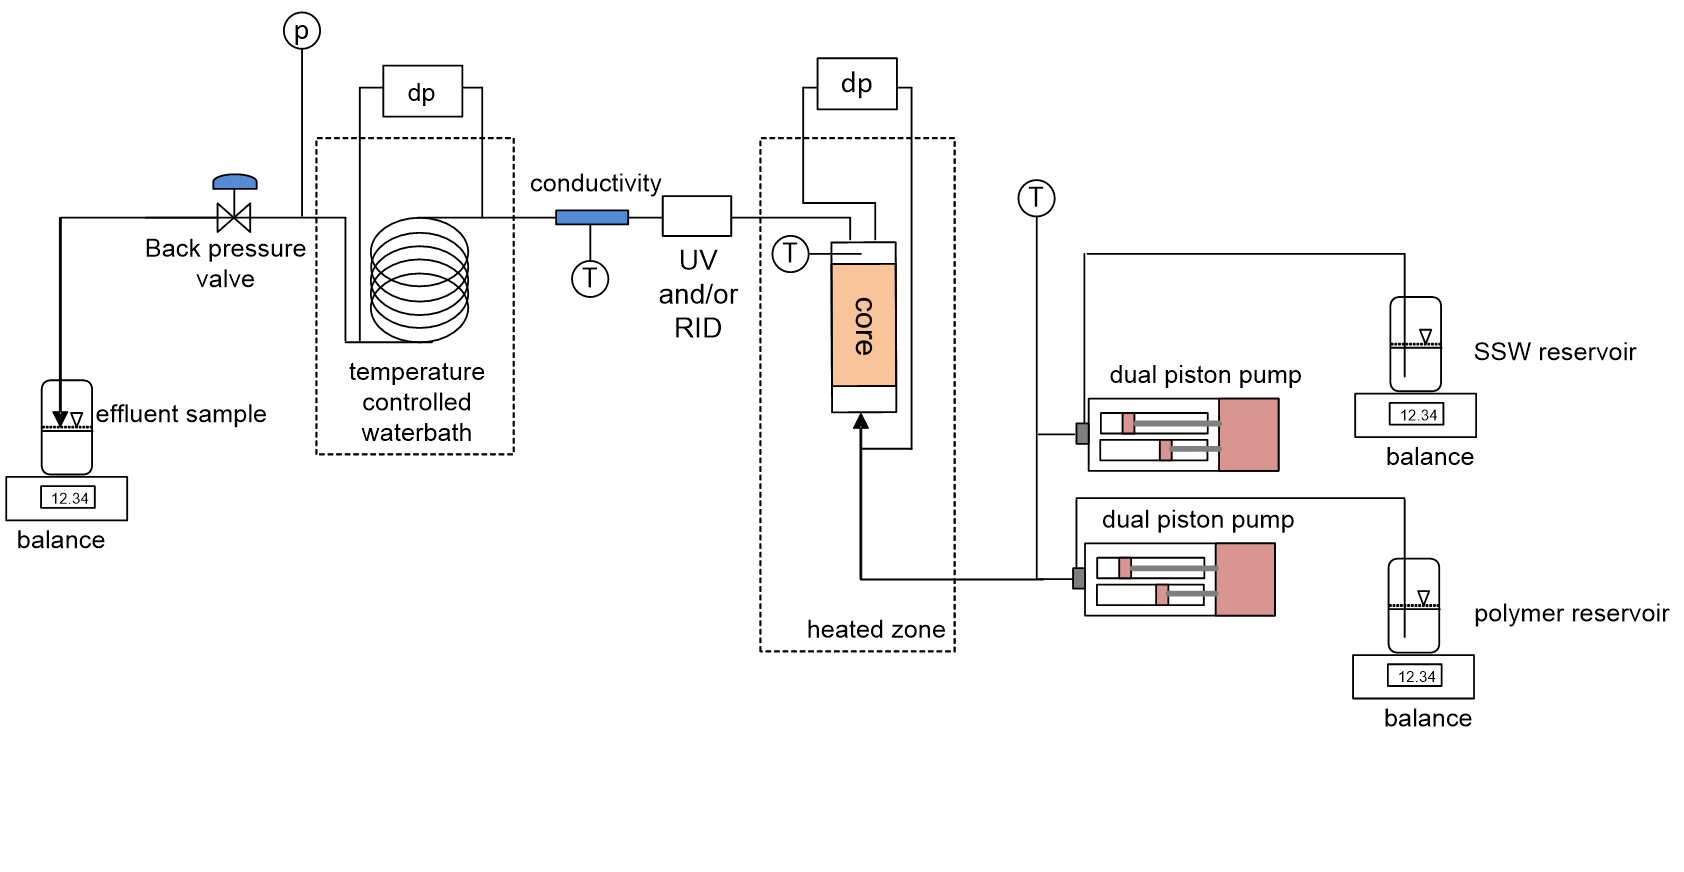
\includegraphics[width=\textwidth]{fig/experimentalSetup.png}
        \caption{Schematic of the setup of the core flooding experiments.}
        \label{fig:experimentalSetup}
    }
\end{figure}

The Bentheimer cores were initially characterized by measurement of porosity and permeability. Pore size distribution was not measured for the present cores. However, from previous measurements with Bentheimer sandstones with the same porosities, a pore size distribution curve was determined based on mercury intrusion measurements as shown in Figure \ref{cht:poreSizeDist}. The maximum of the curve was 33 \micro m, and only 11 \% of the pore throats were less than 10 \micro m (as seen from the raw data underlying the distribution curve).

\begin{figure}
    \centering
    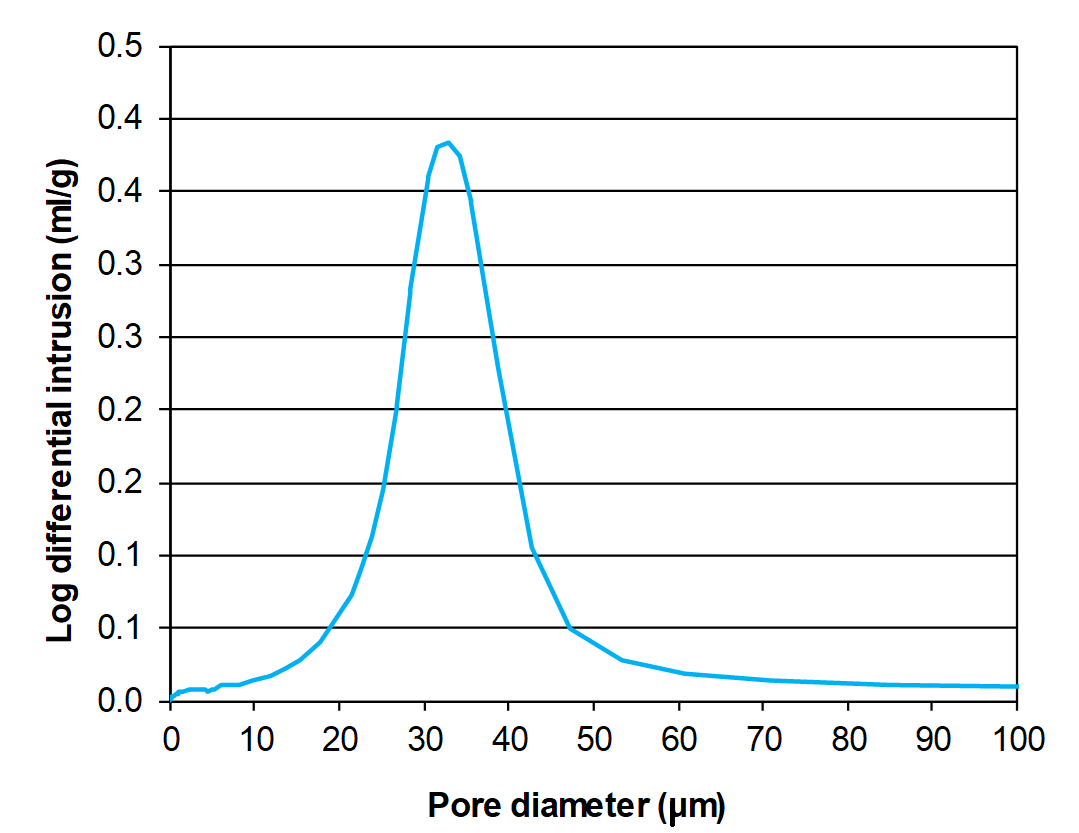
\includegraphics[width=.7\textwidth]{fig/poreSizeDist.png}
    \caption{Pore size distribution for Bentheimer sandstone}
    \label{cht:poreSizeDist}
\end{figure}

In total, three experiments were conducted with increasing aging times for the chemical system in the core. For each experiment, the pore volume and absolute permeability was first measured. Then, the chemical system was injected, followed by aging. After aging, SSW was injected at 30 ml/hr, and the experiments ended with a permeability measurement. During injection of the chemical system, samples of the produced fluid were taken early after breakthrough of the chemicals and at the end of the injection.
The SSW injected prior to the polymer/nanoparticle solution was purged with argon and vacuum treated to remove oxygen from the solutions.


% \section{Transport of polymer and nanoparticles through porous media}
% \subsection{Experimental setup}
% A schematic of the experimental setup is shown in Figure \ref{fig:experimentalSetup}. To the right of the setup there were reservoirs containing either SSW, nanoparticle solution, polymer solution or mixtures of the latter two. The solutions were then pumped by a dual piston Pharmacia P-500 pump, and injected into the bottom of the vertical oriented core. The core itself was wrapped in nickel foil and inserted into a Viton rubber sleeve, around which a net overburden pressure of 50 bar was exerted. This ensured that no side flow occurred around the core and the metal foil prevented the sleeve pressure gas to diffuse through rubber sleeve.

% \begin{figure}[hp]
%     \adjustbox{minipage=\textheight,angle=90}{
%         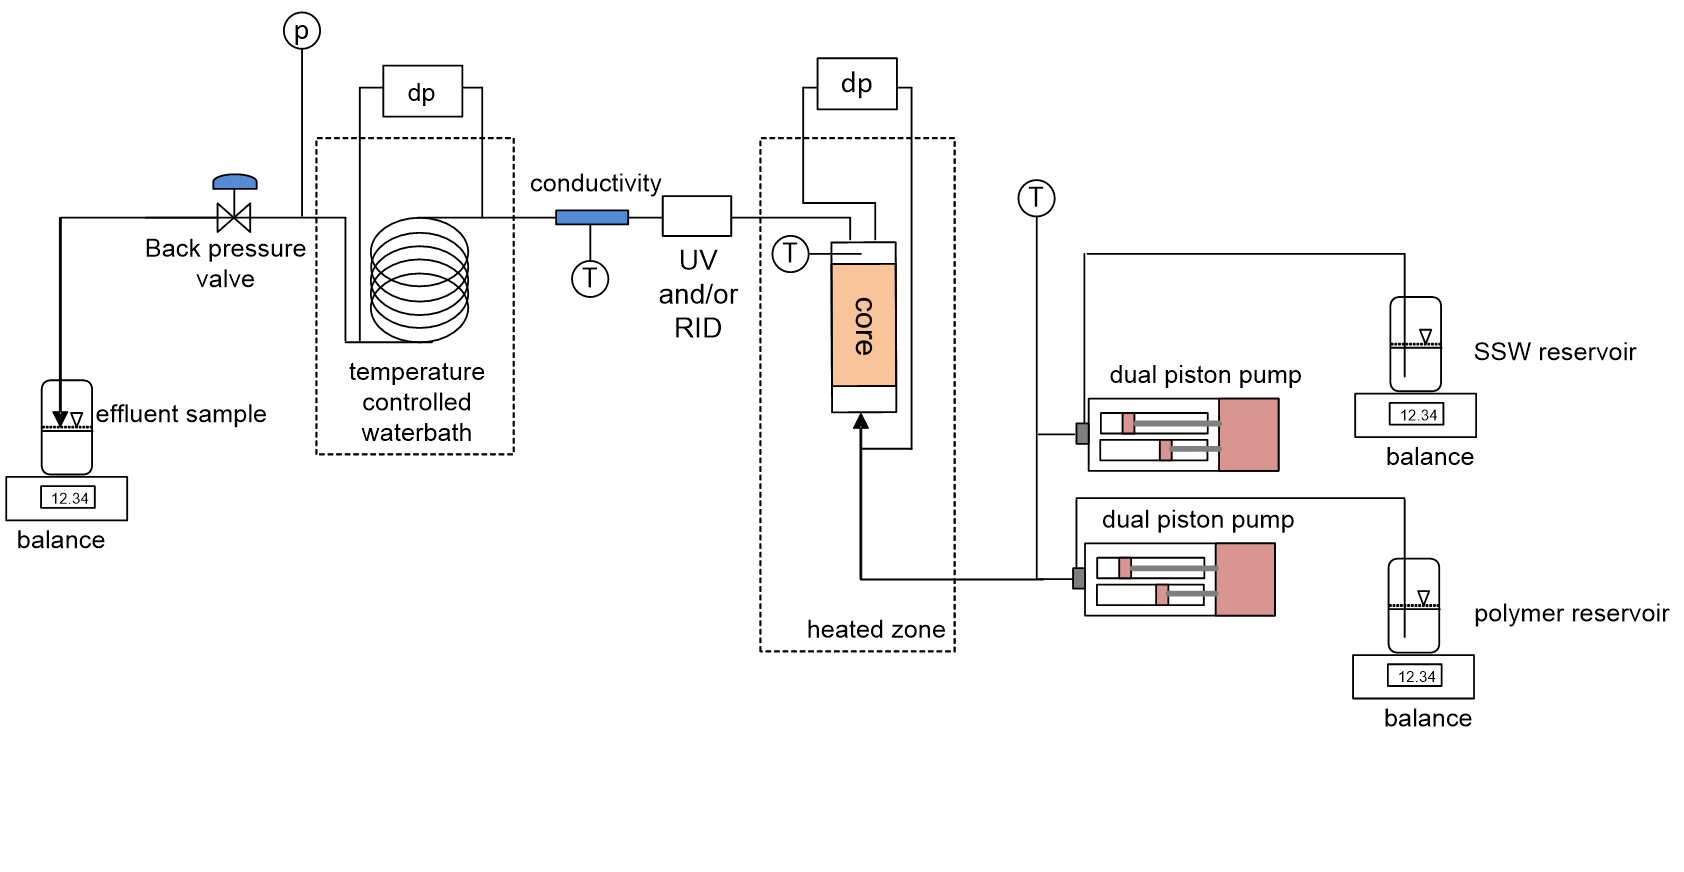
\includegraphics[width=\textwidth]{fig/experimentalSetup.png}
%         \caption{Schematic of the setup of the core flooding experiments.}
%         \label{fig:experimentalSetup}
%     }
% \end{figure}

% Several online measurement systems were placed downstream of the core. Conductivity of the effluent was measured by a Radiometer CDM 83 Conductivity Meter, determining the resistance of the fluid between two small rodded platinum electrodes integrated in a flow channel in a small housing made of polyoxymethylene. Since conductivity is substantially affected by temperature, these readings were temperature corrected. Viscosity of the effluent was measured by a spiral viscometer of 1/16" outer diameter. In order to avoid temperature effects, the viscometer was submerged in a water bath with a constant temperature. A refractive index detector (Shodex RI SE-51) and UV detector (KNAUER Azura MWD 2.1L) were employed interchangeably, in order to determine nanoparticle concentration. Several pressure transducers were implemented along the system. A back pressure of 3 – 6 bar was applied. To the left side of the experimental setup, the effluents were collected and weighed. The core temperature was at ambient for the experiments described in this section.

% \subsection{Core flooding experiments with polymer and/or inactive FN particles}

% First, a new core of diameter 3.8 cm and length 20 cm, was mounted in the core holder. After leakage testing of the system, the core was flooded with isopropanol until full saturation. Next several PVs of synthetic seawater (SSW) were flooded through the core in order to displace the isopropanol and ensure stable flow conditions. After that, porosity and permeability measurements were conducted. Porosity was measured by NaNO3 flooding of the SSW saturated core. The concentration of \ce{Cl-} in the collected fluid was determined by potentiometric titration. The pore volume (PV) was calculated from the total amount of chloride, adequately corrected for dead volumes.

% Each experiment started with injection of a slug with only nanoparticles, only polymer or a mixture of nanoparticles and polymer (Stage 1). After some time, the measurements stabilised. In Stage 2, the injected fluid was switched to pure brine (with lower salt concentration in the experiments only involving polymer) and the injection continued until the measurements became stable. In Stage 3, a second slug with additives was injected, followed by a second slug with only brine (Stage 4). In other words, stages 3 and 4 were a repetition of stages 1 and 2. All stages ran until measurements became steady state. The experiment ended with a final water permeability measurement. During the experiment, process parameters and detector/sensor readings were continuously logged.

% Quantification of produced polymer and nanoparticles was carried out using the viscosity measurements and/or measured changes in refractive index and UV absorption. Figure \ref{cht:uv} shows calibration models for UV absorption and pressure drop in the viscometer tube. As seen in the figure, the pressure drop over viscometer tube is practically only affected by polymer concentration, giving a second order model in polymer concentration. Viscosity measurements alone were therefore used to find the concentration of produced polymer. On the other hand, UV absorption data resulted in a model with first and second order terms with respect to both nanoparticles and polymer, as well as a cross term (i.e., the product of concentrations). Similar responses were also found for changes in refractive index. UV absorption measurements and changes in refractive index were used to generate nanoparticle responses. For the experiments that involved nanoparticles, the conductivity responses were determined in separate runs from the main core floods. This was because changes in salt concentration affected both UV absorption at low wavelengths and especially the refractive index of the fluid. The conductivity responses were measured with the same injection rates with slugs of SSW and 80\% SSW into the cores.

% \begin{figure}[h]
%     \centering
%     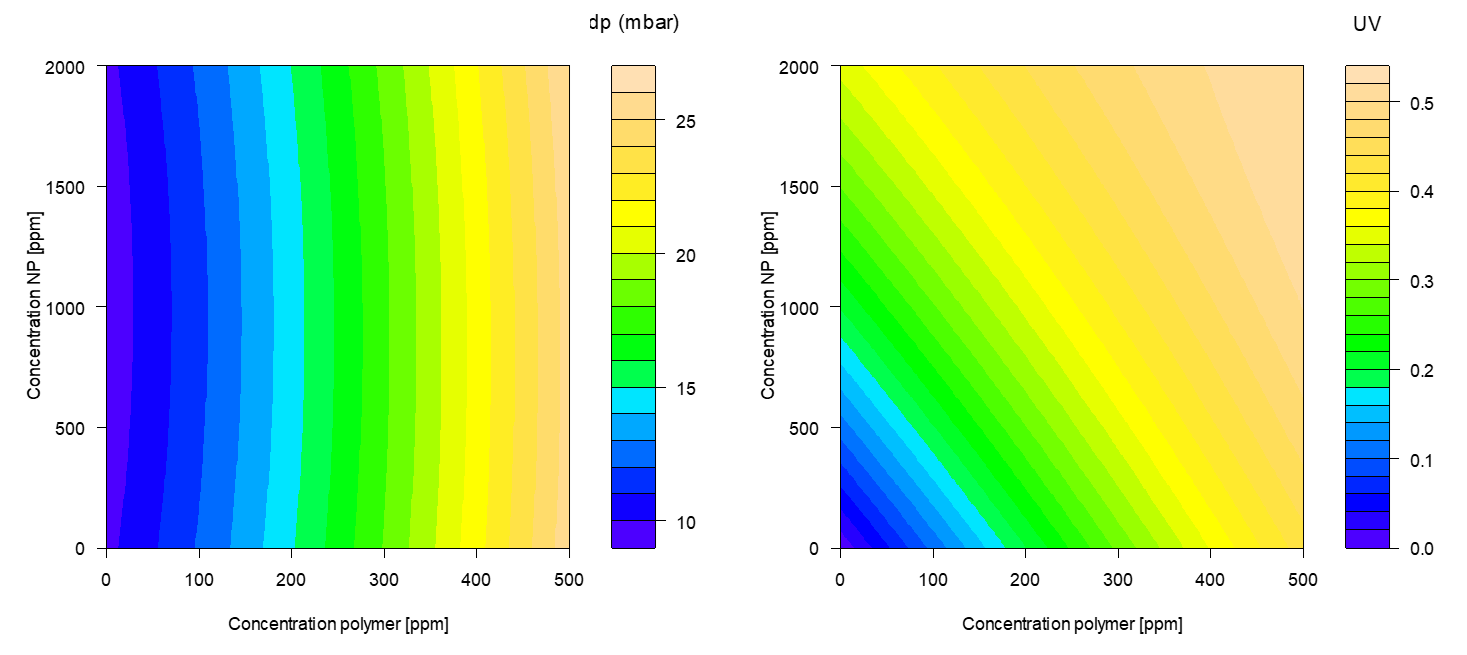
\includegraphics[width=\textwidth]{fig/uvDetector.png}
%     \caption{Calibration models for pressure drop in viscometer (left) and UV absorption in UV detector (right). Polymer concentration varies along the horizontal axis and nanoparticle concentration varies along the vertical axis.}
%     \label{cht:uv}
% \end{figure}

% Online measurements of polymer and nanoparticles using UV and refractive index measurements proved to be difficult. The reason for this is not revealed, but staining of the flow cells in the instruments is believed to be the most likely cause of these problems that also affected the accuracy in the results.

% Nanoparticle and polymer solutions were prepared with synthetic SSW as solvent. Table \ref{tab:rockParams} summarizes the six different additive combinations used. Some of the experiments were repeated. Table \ref{tab:sswComp} shows the recipe for SSW used. In order to make a nanoparticle solution, Funzio-nano particles (FN-PEGMEA-100-141128) produced at SINTEF Materials and Chemistry were dissolved in SSW using a magnetic stirrer and then exposed to ultra-sonic bath a better dissolution. Finally, the solution was filtered through a 0.45 µm membrane filter. No significant increase in mass of the filters were detected. Partially hydrolyzed polyacrylamide (HPAM, FP 5115 VHM from SNF Floerger) was employed as the polymer. The molecular weight of the polymer is not exactly known but assumed in the order of 12 - 15 MDa. HPAM powder was dissolved in SSW with a propeller at 500 rpm followed by magnetic stirring. The polymer solutions, either at working concentrations or more concentrated solutions, were filtered through 5 cm long 500 mD Berea cores at rates up to 16 ml/min, but avoiding differential pressures over 20 bar. Two types of sandstone were used; Berea and Bentheimer. Basic core parameters are given in Table \ref{tab:rockParams}.

% \begin{table} 
% \small
% \centering
% \caption{Basic rock parameters and additives used in the experiments.}
% \label{tab:rockParams}
% \begin{tabular}{c c c c l } 
% \toprule
% \textbf{Exp. no.} & \textbf{Rock} & \textbf{Permeability} & \textbf{Porosity} & \textbf{Additive} \\ 
% && [Darcy] & [\%] & \\
% \midrule 
% 1   & Bentheimer    & 2.74 & 23.1 & Nanoparticles\\
% 2   & Bentheimer    & 2.81 & 23.1 & Polymer \\ 
% 3   & Bentheimer    & 2.84 & 23.5 & Nanoparticles \& Polymer \\ 
% 4   & Berea      & 0.365 & 19.7 & NanoParticles\\
% 5   & Berea      & 0.288 & 18.6 & Polymer \\ 
% 5   & Berea      & 0.359 & 19.7 & Nanoparticles \& Polymer \\ 
% \bottomrule
% \end{tabular}
% \end{table}


% % % %%%%%%%%%%%%%%%%%%%%%
% % % RESULTS
\section{Results}
\textbf{Gel Formation Experiments.} Table \ref{tab:crGelsAt} shows the lowest concentration for gel formation with the different polymers used in the experiments. As seen the table, gel was only formed with Alcoflood 254 S for the highest concentration tested, namely 2 wt. \%. However, it is possible that gels could have been formed at lower concentrations in the interval between 1 wt. \% and 2 wt. \%. Alcomer 24 UK formed gel at 0.5 wt. \% but not at 0.25 wt. \%. It is possible that the highest molecular weight polymer Flopaam 5115 VHM could have formed gels at concentrations lower than 0.5 wt. \%.

In order to obtain data for testing of the simulator \--- developed for transport of nanoparticles and polymer, and with a functionality of time delayed gel formation \--- some gel formation experiments were conducted where the polymer concentration was varied from 0.25 wt. \% to 1 wt. \% and the concentration of \ce{Cr^{3+}} was varied from 22 ppm to 113 ppm. For this series of experiments, Alcomer 24 UK was used as polymer. For concentrations higher than 22 ppm, the polymer viscosity was apparently not dependent on the cross-binder concentration (within the accuracy of the measured viscosities as discussed before). The viscosities of the solutions were measured directly after preparation and after one day of aging. Figure \ref{cht:viscAlco} shows viscosity as function of shear rate for three polymer concentrations. 
\begin{figure}
    \centering
    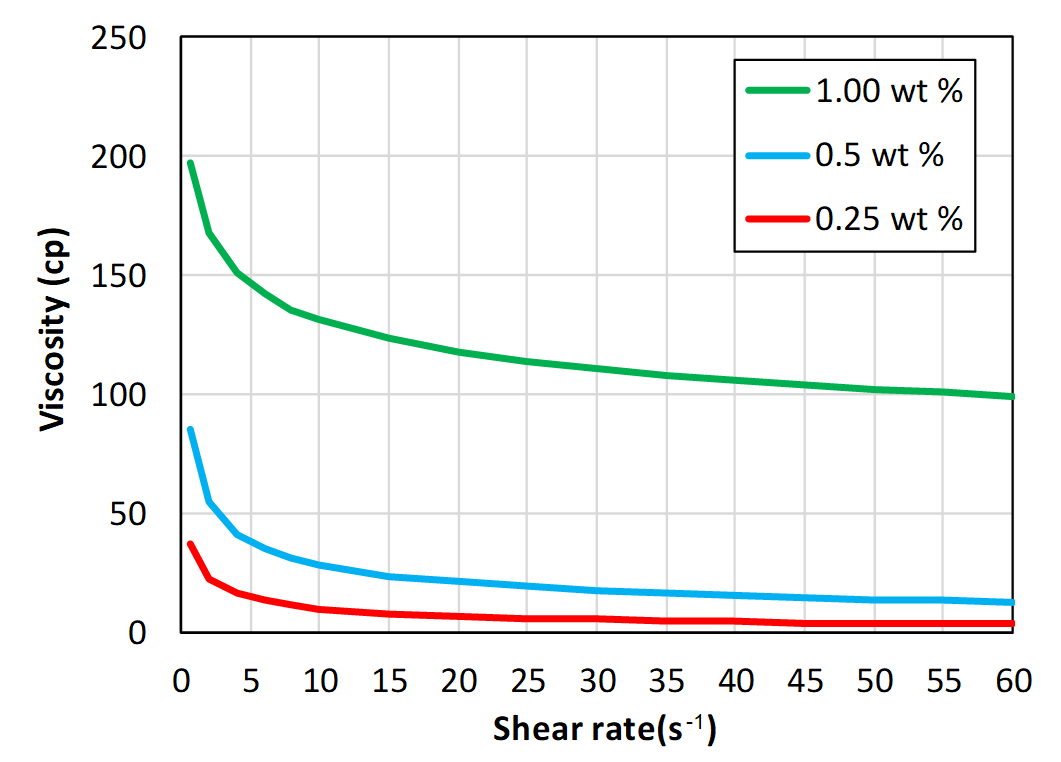
\includegraphics[width=.75\textwidth]{fig/viscAlcomer.png}
    \caption{Viscosity as function of shear rate and polymer concentration for Alcomer 24 UK}
    \label{cht:viscAlco}
\end{figure}

\begin{table}[h]
\small
\centering
\caption{Minimum concentration for gel formation for the different polymers}
\label{tab:crGelsAt}
\begin{tabular}{c c c c >{\columncolor[gray]{0.8}}c } 
\toprule
\textbf{Name} & \textbf{Producer} & \textbf{MW} & \textbf{Concentration} & \textbf{Will gel at} \\ 
&& [MDa] & [wt\%] & [wt\%]  \\
\midrule 
Alcoflood 254 S     & BASF    & 0.5 & 0.5, 1.0 and 2.0 & 2\\
Alcomer 24 UK       & BASF    & 6 & 0.25, 0.5, 1.0 and 2.0 & $\geq 0.5$ \\ 
Flopaam 5115 VHM    & SNF Floerger    & 12+ & 0.5, 1.0 and 2.0 & $\geq 0.5$ \\ 
\bottomrule
\end{tabular}
\end{table}

Figure \ref{cht:viscPolcModel} shows an example of a reaction model designed based on viscosities measured at a shear rate of 12.7 s$^-1$ for the fresh made solutions and after one day of aging. The blue curve corresponds to the polymer which has not reacted, i.e. data taken from Figure \ref{cht:viscAlco}. It also corresponds to the viscosities for aging times less than 50 days with reference to Figure \ref{cht:jennTai} (although some viscosity increase was seen in this period). The red curve corresponds to maximum viscosities for the solutions, corresponding to the value after 60 days in Figure \ref{cht:jennTai} that is only valid for a single polymer concentration. The green curve is for aging time laying between no gelling and complete gelling. Again, with reference to Figure \ref{cht:jennTai} the green curve would be valid for an aging time of 55 days. In the reaction model, it is assumed that the viscosity increases linearly with time in the gelling period. Again, as mentioned above, the reaction model was solely made to have some reality based data to be used for testing of the simulator model. 

\begin{figure}
    \centering
    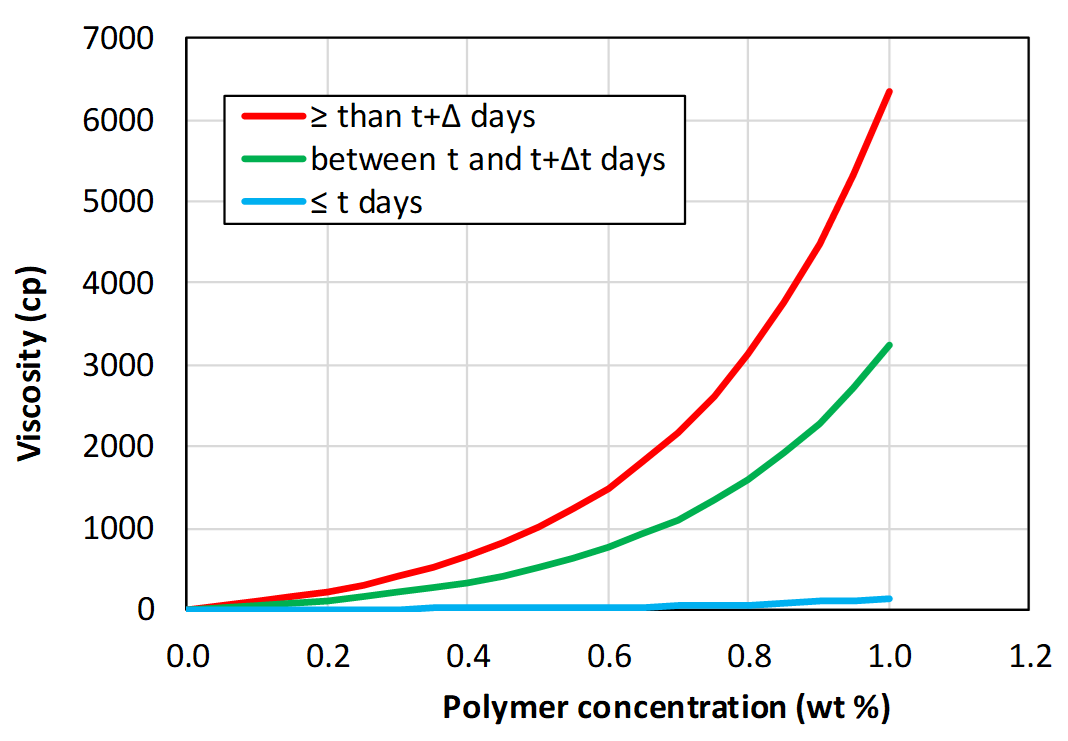
\includegraphics[width=.75\textwidth]{fig/viscPolcModel.png}
    \caption{Reaction model for Alcomer 24 UK}
    \label{cht:viscPolcModel}
\end{figure}

\textbf{In situ Gelling Experiments.}
Table \ref{tab:porPermAge} summarises the initial absolute permeabilities of the cores used in the experiments, the permeabilities measured after the SSW injections and the residual resistance factors, i.e. the ratio between the two permeabilities. The resistance factor determined after 7 days of aging was not much higher than the corresponding factor determined for polymer injection into Bentheimer sandstone, cf. Figure 5.20. As illustrated by the figure, the residual resistance factors increased with longer aging times.
%TAB
\begin{table}
\small
\centering
\caption{Porosities, initial and final permeabilities and residual resistance factor for various aging times.}
\label{tab:porPermAge} % 5.12
\begin{tabular}{c l l l l l } 
\toprule
\textbf{Exp. no.} & \textbf{Porosity} & \textbf{Aging time} & \textbf{Abs. perm.} & \textbf{Residual perm.} & \textbf{RRF} \\ 
 & [fraction] & [days] & [mD] & [mD] & \\
\midrule 
1  & 0.221   &  7     & 2653     & 306      & 8.7    \\
2  & 0.221   & 23     & 2580     & 5.2      & 493      \\ 
3  & 0.221   & 66     & 2706     & 0.008    & 3230   \\ 
\bottomrule
\end{tabular}
\end{table}

The injection phases for the nanoparticle/polymer solution are compared in Figure \ref{cht:gelexp_sum}. As seen the differential pressures across the viscometer tube were similar. In Experiment 3 parts of the bypass line was filled with the nanoparticle/polymer mixture, explaining the initial decline in the viscosity response. 

\begin{figure}[h!]
    \centering
    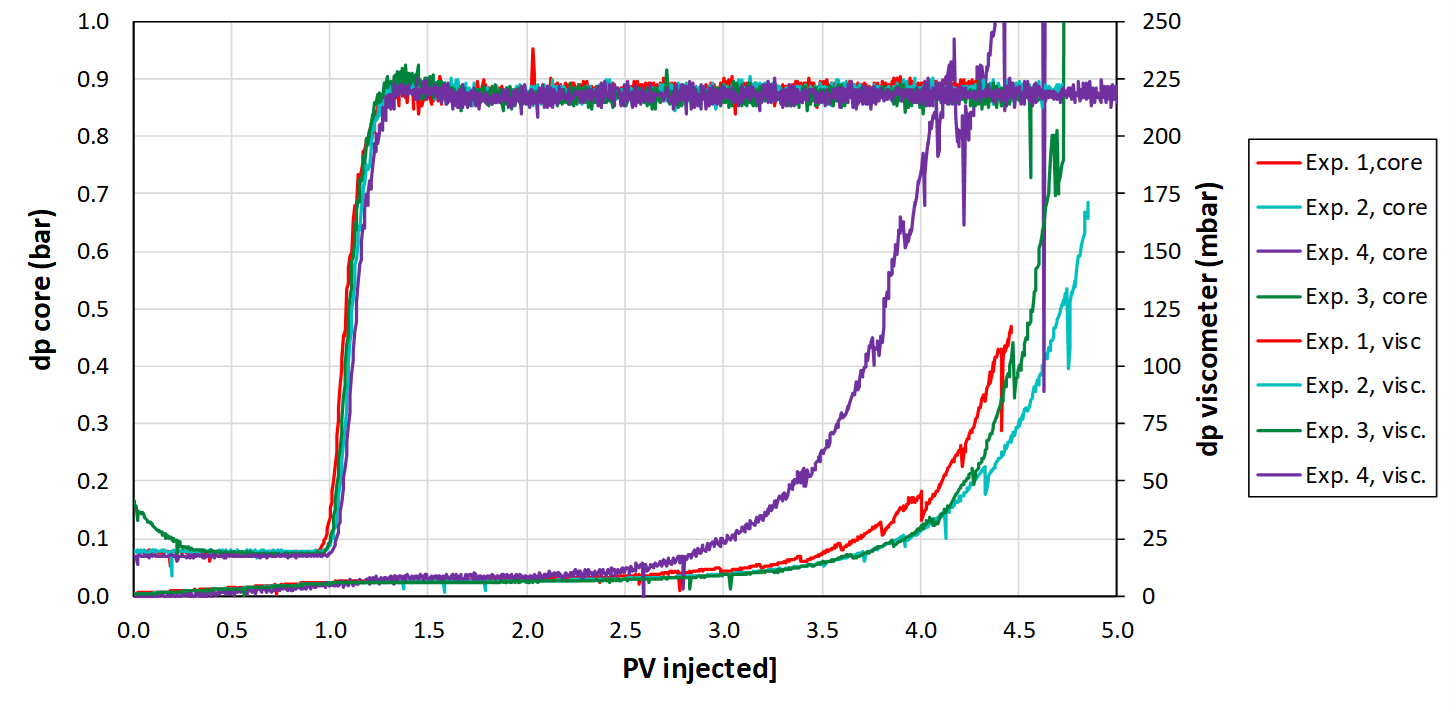
\includegraphics[width=\textwidth]{fig/gelexp_sum.png}
    \caption{Comparison of nanoparticle/polymer injection phases.}
    \label{cht:gelexp_sum} % 5.39
\end{figure}
 
The differential pressures over the core developed almost identical for the first 2.5 PVs injected. The rapid increase thereafter, developed in different, but quite similar manners. Filtering through a core apparently gave a less good pre-filtering of the solution compared to filtration through 8 \micro m membrane filters.

If the presence of extended structures/particles in the solution is the cause of the injectivity problem, the use of finer filters, possibly in combination with ultrasonication, could alleviate the problem.

The experiments with in situ gelling has demonstrated that gel is formed in the porous medium. As expected the gel strength increases with increased gelling time. For a gelling time, somewhat longer than 2 months, a strong gel was formed. This gel almost blocked the core with a pressure gradient of 135 bar/m for almost 9 days, but injected SSW could only flow for still large pressure gradients across the core. The residual resistance factor after 75 PV injected was still 3230.




% back matter
\newpage
\bibliography{ref}
\end{document}


